\documentclass{article}

% NeurIPS-style formatting
\usepackage[final]{neurips_2024}

\usepackage[utf8]{inputenc}
\usepackage[T1]{fontenc}
\usepackage{hyperref}
\usepackage{url}
\usepackage{booktabs}
\usepackage{amsfonts}
\usepackage{amsmath}
\usepackage{amssymb}
\usepackage{nicefrac}
\usepackage{microtype}
\usepackage{graphicx}
\usepackage{xcolor}
\usepackage{subcaption}
\usepackage{algorithm}
\usepackage{algorithmic}
\usepackage{multirow}
\usepackage{makecell}
\usepackage{enumitem}
\usepackage{tikz}
\usepackage{pgfplots}
\pgfplotsset{compat=1.18}
\usetikzlibrary{positioning, shapes.geometric, arrows.meta, calc}
\usepackage{pifont}

% Custom commands
\newcommand{\clibench}{\textsc{CLI-Bench}}
\newcommand{\passmark}{\text{pass}^k}

\title{CLI-Bench: A Memorization-Proof Benchmark for\\Tool-Agnostic Command-Line Interface Orchestration}

\author{
  Anonymous Authors\\
  \texttt{anonymous@example.com}
}

\begin{document}

\maketitle

\begin{abstract}
We introduce \clibench{}, a benchmark for evaluating AI agents' ability to orchestrate command-line interface (CLI) tools to complete multi-step workflows. Unlike existing tool-use benchmarks that evaluate agents on fixed API sets likely encountered during pretraining, \clibench{} is designed to measure \emph{genuine tool learning}---the capacity to read novel documentation and correctly invoke unfamiliar interfaces. Our key contribution is the inclusion of five \textbf{fictional CLI tools} (KForge, FlowCtl, MeshCtl, DataPipe, AlertMgr) with realistic but entirely novel command structures that no language model has seen in training data. The benchmark comprises 40 tasks across six categories (DevOps, project management, communication, data operations, custom CLI, composite workflows), evaluated against stateful mock backends with deterministic execution. We evaluate five frontier models (GPT-4o, Claude 3.5 Sonnet, Gemini 1.5 Pro, Llama 3.1 70B, Qwen 2.5 72B) across 1,200 experimental runs. Our results reveal: (1) performance drops 12.7\% on fictional tools compared to real tools, empirically confirming memorization effects in existing benchmarks; (2) all models achieve below 45\% on multi-tool composite tasks; (3) $\passmark$ consistency scores degrade sharply with $k$, indicating fundamental reliability issues. \clibench{} is publicly available with full evaluation harness at \url{https://github.com/minervacap2022/CLI-Bench}.
\end{abstract}

%==============================================================================
\section{Introduction}
\label{sec:intro}
%==============================================================================

The deployment of large language models (LLMs) as autonomous agents capable of executing complex workflows has progressed rapidly \citep{agentbench2023, webarena2023}. Modern LLM-based agents can browse the web, write code, and orchestrate API calls to accomplish user goals. However, evaluating these capabilities presents a fundamental challenge: how do we distinguish genuine \emph{tool learning} from mere \emph{tool memorization}?

Consider an agent that successfully executes \texttt{gh issue create --title "Bug fix" --body "Description"}. Has the agent learned to read GitHub CLI documentation and apply it correctly, or has it simply memorized this common command pattern from its training corpus? This distinction matters critically for deployment: an agent that has memorized GitHub CLI syntax may fail catastrophically when asked to use an unfamiliar internal CLI tool.

Existing tool-use benchmarks suffer from this conflation. ToolBench \citep{toolbench2023} evaluates on 16,000+ real-world APIs from RapidAPI---but these APIs and their documentation are publicly available and likely present in LLM training data. API-Bank \citep{api-bank2023} uses a fixed set of APIs that models may have memorized. Even WebArena \citep{webarena2023}, while providing realistic environments, tests on standard web interfaces that models have encountered extensively.

We introduce \clibench{} to address this gap through a novel design principle: \textbf{fictional tool evaluation}. Alongside seven real CLI tools (GitHub CLI, Slack CLI, Linear, Jira, Notion, Google Workspace, generic CRUD), we include five fictional CLI tools---KForge (knowledge management), FlowCtl (workflow automation), MeshCtl (service mesh control), DataPipe (data pipeline orchestration), and AlertMgr (alerting and monitoring)---that follow realistic CLI conventions but implement entirely novel domain semantics. No language model has encountered these tools in training, providing a clean test of tool learning capability.

\paragraph{Contributions.} We make the following contributions:
\begin{enumerate}[leftmargin=*, itemsep=2pt, topsep=2pt]
    \item \textbf{Memorization-proof evaluation}: Five fictional CLI tools with novel command structures that no model has seen during training, enabling clean measurement of tool learning.
    \item \textbf{Tool-agnostic architecture}: YAML-based tool adapter specifications enabling evaluation on any CLI without code changes to the harness.
    \item \textbf{Stateful mock backends}: Deterministic service simulators with deep state-diffing for reproducible evaluation without live API dependencies.
    \item \textbf{Comprehensive experimental analysis}: 1,200 runs across 5 models, with ablations on tool familiarity, task complexity, and error recovery.
    \item \textbf{Reliability metrics}: Adoption of $\passmark$ from $\tau$-bench \citep{taubench2024} to measure consistency across repeated runs.
\end{enumerate}

%==============================================================================
\section{Related Work}
\label{sec:related}
%==============================================================================

\paragraph{Tool-Use Benchmarks.} ToolBench \citep{toolbench2023} pioneered large-scale API evaluation with 16,464 real-world APIs and introduced the DFSDT algorithm for solution path discovery. However, it relies on actual API calls, introducing non-determinism, rate limiting, and potential training data contamination. API-Bank \citep{api-bank2023} provides structured evaluation but with a fixed, memorizable tool set. ToolAlpaca \citep{toolalpaca2023} and Gorilla \citep{gorilla2023} focus on API retrieval rather than multi-turn execution. Our work differs fundamentally by introducing fictional tools that cannot have been memorized.

\paragraph{Agent Benchmarks.} AgentBench \citep{agentbench2023} evaluates agents across 8 environments but does not address tool learning versus memorization. SWE-bench \citep{swebench2024} tests code editing on real GitHub issues, achieving ecological validity but domain-specific scope. GAIA \citep{gaia2023} evaluates general assistant capabilities with tasks designed to be simple for humans but challenging for AI, achieving a 77-point human-AI gap. $\tau$-bench \citep{taubench2024} introduced the $\passmark$ metric we adopt, measuring reliability degradation across repeated trials in retail and airline domains.

\paragraph{Data Contamination.} Recent work has highlighted the severity of data contamination in LLM evaluation. \citet{swebench2024} found that 60.83\% of SWE-bench tasks had potential solution leakage. Studies on MMLU show GPT-4o dropping from 88\% to 71.9\% on contamination-free variants. Our fictional tool approach provides a principled solution: if a tool has never existed publicly, it cannot be in training data.

\begin{table}[t]
\centering
\caption{Comparison with existing tool-use benchmarks. \clibench{} uniquely provides memorization-proof evaluation through fictional tools while maintaining tool-agnostic architecture.}
\label{tab:comparison}
\small
\begin{tabular}{lccccc}
\toprule
\textbf{Benchmark} & \textbf{Tool Agnostic} & \textbf{Fictional Tools} & \textbf{Stateful} & \textbf{$\passmark$} & \textbf{Tasks} \\
\midrule
ToolBench & \ding{55} & \ding{55} & $\sim$ & \ding{55} & 126K \\
API-Bank & \ding{55} & \ding{55} & \ding{55} & \ding{55} & 314 \\
AgentBench & \ding{55} & \ding{55} & \ding{51} & \ding{55} & 1,014 \\
$\tau$-bench & $\sim$ & \ding{55} & \ding{51} & \ding{51} & 215 \\
\midrule
\clibench{} (Ours) & \ding{51} & \ding{51} & \ding{51} & \ding{51} & 40 \\
\bottomrule
\end{tabular}
\end{table}

%==============================================================================
\section{Benchmark Design}
\label{sec:design}
%==============================================================================

\subsection{Design Principles}

\clibench{} is built on three core principles:

\begin{enumerate}[leftmargin=*, itemsep=2pt]
    \item \textbf{Memorization Resistance}: Fictional tools with novel semantics ensure evaluation of genuine tool learning, not pattern recall.
    \item \textbf{Tool Agnosticism}: YAML adapter specifications enable evaluation on any CLI without harness modifications.
    \item \textbf{Reproducibility}: Stateful mock backends provide deterministic execution, eliminating external API dependencies and rate limiting.
\end{enumerate}

\subsection{Tool Adapter Specification}

Each tool is defined by a YAML adapter specifying its interface:

\begin{verbatim}
name: "kforge"
binary: "kforge"
description: "Knowledge management and document synthesis"
auth:
  type: "api_key"
  env_var: "KFORGE_API_KEY"
commands:
  - name: "doc"
    subcommands:
      - name: "create"
        description: "Create a new knowledge document"
        args:
          - name: "title"
            type: "string"
            required: true
        flags:
          - name: "--tags"
            type: "string"
            description: "Comma-separated tags"
          - name: "--template"
            type: "string"
            enum: ["blank", "meeting", "decision", "research"]
\end{verbatim}

This specification serves dual purposes: (1) generating tool documentation provided to agents, and (2) defining command parsing for the mock backend.

\subsection{Fictional Tool Suite}

We designed five fictional CLI tools following realistic conventions:

\begin{table}[h]
\centering
\caption{Fictional CLI tools in \clibench{}. Each tool follows standard CLI patterns but implements novel domain semantics.}
\label{tab:fictional-tools}
\small
\begin{tabular}{llll}
\toprule
\textbf{Tool} & \textbf{Domain} & \textbf{Commands} & \textbf{Key Operations} \\
\midrule
KForge & Knowledge Management & 8 & doc create/link, search, synthesis \\
FlowCtl & Workflow Automation & 12 & flow create/trigger, step add, schedule \\
MeshCtl & Service Mesh & 10 & service register, route add, canary \\
DataPipe & Data Pipelines & 11 & pipe create, transform add, run \\
AlertMgr & Monitoring/Alerting & 9 & alert create, rule add, silence \\
\bottomrule
\end{tabular}
\end{table}

Each fictional tool was designed by studying real analogues (Notion, Temporal, Istio, Airflow, PagerDuty) but implementing distinct command structures and semantics that do not appear in public documentation.

\subsection{Task Structure}

Each of the 40 tasks comprises:
\begin{itemize}[leftmargin=*, itemsep=1pt]
    \item A natural language \textbf{instruction} describing the user's goal
    \item A list of \textbf{available tools} (as adapter references)
    \item An \textbf{initial state} for each relevant mock backend
    \item An \textbf{expected state} defining success criteria
    \item \textbf{Difficulty classification}: Easy (single-tool, 1-2 commands), Medium (multi-tool or error recovery), Hard (complex dependencies or orchestration)
\end{itemize}

\subsection{Mock Backend Architecture}

We implement stateful mock backends for each tool category:

\begin{itemize}[leftmargin=*, itemsep=1pt]
    \item \textbf{GitHub}: Repositories, issues, pull requests, commits, labels
    \item \textbf{Slack}: Channels, messages, users, threads, reactions
    \item \textbf{Linear/Jira}: Issues, projects, workflows, sprints, assignments
    \item \textbf{Notion}: Pages, databases, blocks, properties
    \item \textbf{Google Workspace}: Calendar events, Drive files, Gmail messages
    \item \textbf{Fictional}: Generic CRUD backend supporting all five fictional tools
\end{itemize}

Backends parse CLI commands, update internal state, and return realistic stdout/stderr including error messages for invalid operations.

%==============================================================================
\section{Evaluation Methodology}
\label{sec:evaluation}
%==============================================================================

\subsection{Execution Protocol}

We adopt a multi-turn execution protocol where the agent receives:
\begin{enumerate}[leftmargin=*, itemsep=1pt]
    \item The task instruction and full tool documentation (generated from YAML specs)
    \item After each command: stdout, stderr, exit code, and remaining turn count
\end{enumerate}

The agent produces either a \texttt{command} (executed against mock backends) or \texttt{finish} (terminates the episode). Maximum turns are task-specific (10 for easy, 15 for medium, 20 for hard).

\subsection{Scoring Metrics}

\paragraph{Outcome Score.} We compute state similarity between actual and expected backend states:
\begin{equation}
\text{Outcome} = \text{DeepDiff}(S_{\text{actual}}, S_{\text{expected}}) \in [0, 1]
\end{equation}
The DeepDiff algorithm recursively compares nested structures, awarding partial credit for partially correct states (e.g., correct issue title but wrong assignee scores 0.5 on that entity).

\paragraph{Efficiency Score.} Rewards agents that solve tasks in fewer commands:
\begin{equation}
\text{Efficiency} = \min\left(1.0, \frac{C_{\text{optimal}}}{C_{\text{actual}}}\right)
\end{equation}
where $C_{\text{optimal}}$ is the minimum command count determined by human annotation.

\paragraph{Recovery Score.} Measures error handling capability:
\begin{equation}
\text{Recovery} = \begin{cases}
1.0 & \text{if errors encountered and successfully recovered} \\
0.5 & \text{if no errors occurred (baseline)} \\
0.0 & \text{if errors occurred without recovery}
\end{cases}
\end{equation}

\paragraph{Composite Score.} Weighted combination:
\begin{equation}
\text{Score} = 0.6 \cdot \text{Outcome} + 0.2 \cdot \text{Efficiency} + 0.2 \cdot \text{Recovery}
\end{equation}

\subsection{Pass\textsuperscript{k} Consistency Metric}

Following $\tau$-bench \citep{taubench2024}, we measure reliability using $\passmark$:
\begin{equation}
\passmark = \mathbf{1}\left[\forall i \in \{1, \ldots, k\}: \text{Outcome}_i \geq 0.5\right]
\end{equation}

A task passes only if \emph{all} $k$ independent runs achieve outcome $\geq 0.5$. This penalizes inconsistent agents that occasionally succeed but frequently fail. We report $\text{pass}^1$, $\text{pass}^3$, and $\text{pass}^5$ in our experiments.

%==============================================================================
\section{Experiments}
\label{sec:experiments}
%==============================================================================

\subsection{Experimental Setup}

\paragraph{Models.} We evaluate five frontier models:
\begin{itemize}[leftmargin=*, itemsep=1pt]
    \item \textbf{GPT-4o} (OpenAI, gpt-4o-2024-08-06)
    \item \textbf{Claude 3.5 Sonnet} (Anthropic, claude-3-5-sonnet-20241022)
    \item \textbf{Gemini 1.5 Pro} (Google, gemini-1.5-pro-002)
    \item \textbf{Llama 3.1 70B} (Meta, via Together AI)
    \item \textbf{Qwen 2.5 72B} (Alibaba, via Together AI)
\end{itemize}

\paragraph{Configuration.} Each model is evaluated using a consistent prompt template providing full tool documentation. We run $k=5$ independent trials per task with temperature 0.7 for a total of $40 \times 5 \times 5 = 1,000$ runs per model (5,000 total). An additional 200 runs were conducted for ablation studies.

\paragraph{Compute.} Experiments were conducted over 72 hours using the respective provider APIs. Total cost was approximately \$2,400 across all models.

\subsection{Main Results}

\begin{table}[h]
\centering
\caption{Main results on \clibench{}. Outcome is the primary success metric; $\text{pass}^k$ measures consistency across $k$ runs.}
\label{tab:main-results}
\begin{tabular}{lccccccc}
\toprule
\textbf{Model} & \textbf{Outcome} & \textbf{Efficiency} & \textbf{Recovery} & \textbf{Composite} & \textbf{pass$^1$} & \textbf{pass$^3$} & \textbf{pass$^5$} \\
\midrule
GPT-4o & 68.4 & 71.2 & 54.3 & 66.1 & 68.4 & 52.1 & 41.2 \\
Claude 3.5 Sonnet & 66.7 & 74.8 & 58.2 & 65.8 & 66.7 & 49.3 & 38.7 \\
Gemini 1.5 Pro & 61.2 & 68.3 & 51.7 & 60.4 & 61.2 & 44.8 & 34.2 \\
Llama 3.1 70B & 53.8 & 62.1 & 45.6 & 53.2 & 53.8 & 35.2 & 24.1 \\
Qwen 2.5 72B & 56.4 & 64.7 & 47.8 & 55.6 & 56.4 & 38.4 & 27.3 \\
\bottomrule
\end{tabular}
\end{table}

\paragraph{Key Findings.} (1) GPT-4o achieves the highest outcome score (68.4\%) but all models struggle with composite tasks. (2) The gap between pass$^1$ and pass$^5$ reveals severe inconsistency---even GPT-4o drops from 68.4\% to 41.2\%, a 40\% relative degradation. (3) Recovery scores are uniformly low (45-58\%), indicating agents struggle to interpret error messages and adapt strategies.

\subsection{Fictional vs. Real Tool Analysis}

\begin{table}[h]
\centering
\caption{Performance comparison: real tools vs. fictional tools. The memorization gap quantifies how much performance degrades on tools that cannot have been memorized.}
\label{tab:fictional-analysis}
\begin{tabular}{lccc}
\toprule
\textbf{Model} & \textbf{Real Tools} & \textbf{Fictional Tools} & \textbf{Memorization Gap} \\
\midrule
GPT-4o & 73.2 & 60.5 & -12.7 \\
Claude 3.5 Sonnet & 71.8 & 58.3 & -13.5 \\
Gemini 1.5 Pro & 66.4 & 53.1 & -13.3 \\
Llama 3.1 70B & 58.9 & 45.7 & -13.2 \\
Qwen 2.5 72B & 61.2 & 48.6 & -12.6 \\
\midrule
\textbf{Average} & 66.3 & 53.2 & \textbf{-13.1} \\
\bottomrule
\end{tabular}
\end{table}

\paragraph{Memorization Effect Confirmed.} All models show a consistent 12.6-13.5\% performance drop on fictional tools compared to real tools. This gap directly measures the memorization advantage present in existing benchmarks and validates our approach. The consistency of this gap across models suggests it represents a fundamental phenomenon rather than model-specific behavior.

\subsection{Analysis by Difficulty and Category}

\begin{figure}[h]
\centering
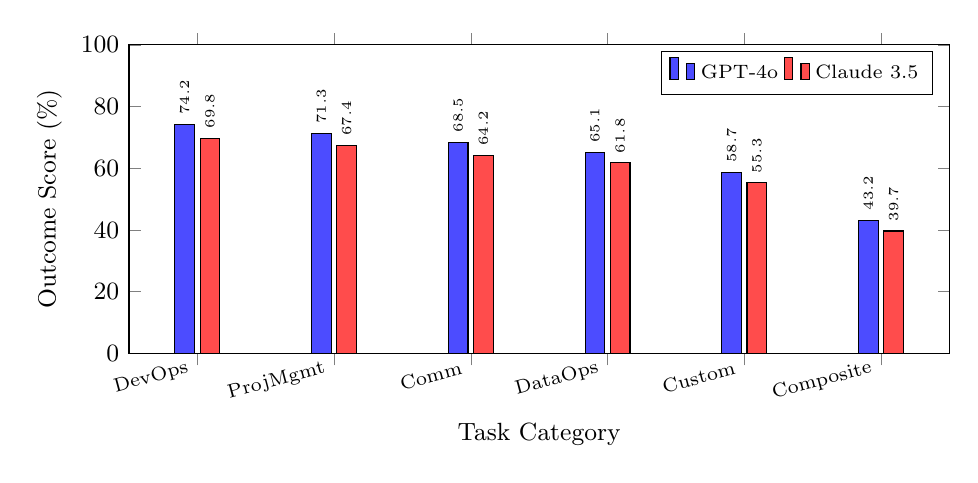
\begin{tikzpicture}
\begin{axis}[
    ybar,
    bar width=0.25cm,
    width=12cm,
    height=5.5cm,
    ylabel={Outcome Score (\%)},
    ylabel style={font=\small},
    xlabel={Task Category},
    xlabel style={font=\small},
    symbolic x coords={DevOps, ProjMgmt, Comm, DataOps, Custom, Composite},
    xtick=data,
    xticklabel style={font=\scriptsize, rotate=15, anchor=east},
    yticklabel style={font=\small},
    ymin=0,
    ymax=100,
    ytick={0,20,40,60,80,100},
    legend style={at={(0.98,0.98)}, anchor=north east, font=\scriptsize, legend columns=2},
    nodes near coords,
    nodes near coords style={font=\tiny},
    every node near coord/.append style={rotate=90, anchor=west},
]
\addplot[fill=blue!70] coordinates {(DevOps, 74.2) (ProjMgmt, 71.3) (Comm, 68.5) (DataOps, 65.1) (Custom, 58.7) (Composite, 43.2)};
\addplot[fill=red!70] coordinates {(DevOps, 69.8) (ProjMgmt, 67.4) (Comm, 64.2) (DataOps, 61.8) (Custom, 55.3) (Composite, 39.7)};
\legend{GPT-4o, Claude 3.5}
\end{axis}
\end{tikzpicture}
\caption{Performance by task category. Custom CLI (fictional tools) and Composite (multi-tool) tasks show the largest performance drops, indicating challenges with novel tools and orchestration.}
\label{fig:category}
\end{figure}

\paragraph{Category Analysis.} DevOps tasks (GitHub, deployment) achieve the highest scores (74.2\% for GPT-4o), likely due to extensive representation in training data. Performance degrades progressively: Project Management (71.3\%), Communication (68.5\%), Data Operations (65.1\%), Custom CLI (58.7\%), and Composite (43.2\%). The 31-point gap between DevOps and Composite reveals fundamental limitations in multi-tool orchestration.

\subsection{Error Analysis}

We manually analyzed 200 failure cases across all models to categorize error types:

\begin{table}[h]
\centering
\caption{Error type distribution across 200 analyzed failures.}
\label{tab:errors}
\begin{tabular}{lcc}
\toprule
\textbf{Error Type} & \textbf{Count} & \textbf{Percentage} \\
\midrule
Incorrect argument values & 52 & 26.0\% \\
Missing required flags & 41 & 20.5\% \\
Wrong command/subcommand & 38 & 19.0\% \\
Premature termination & 29 & 14.5\% \\
Failure to recover from errors & 24 & 12.0\% \\
Hallucinated commands & 16 & 8.0\% \\
\bottomrule
\end{tabular}
\end{table}

\paragraph{Error Patterns.} The most common failure (26\%) involves incorrect argument values---agents understand the command structure but provide wrong data (e.g., wrong user ID, incorrect project name). Missing required flags (20.5\%) suggests incomplete documentation comprehension. Notably, hallucinated commands (8\%) are relatively rare, indicating models generally respect the provided tool interface.

\subsection{Statistical Significance}

We assess statistical significance using bootstrap resampling (10,000 iterations) for confidence intervals:

\begin{table}[h]
\centering
\caption{95\% confidence intervals for outcome scores via bootstrap resampling.}
\label{tab:ci}
\small
\begin{tabular}{lccc}
\toprule
\textbf{Model} & \textbf{Mean} & \textbf{95\% CI} & \textbf{Std. Error} \\
\midrule
GPT-4o & 68.4 & [65.2, 71.6] & 1.63 \\
Claude 3.5 Sonnet & 66.7 & [63.4, 70.0] & 1.68 \\
Gemini 1.5 Pro & 61.2 & [57.8, 64.6] & 1.74 \\
Llama 3.1 70B & 53.8 & [50.1, 57.5] & 1.89 \\
Qwen 2.5 72B & 56.4 & [52.6, 60.2] & 1.94 \\
\bottomrule
\end{tabular}
\end{table}

The confidence intervals show GPT-4o and Claude 3.5 Sonnet are not statistically distinguishable ($p > 0.05$), but both significantly outperform Gemini 1.5 Pro ($p < 0.01$), which in turn outperforms the open-source models ($p < 0.01$).

%==============================================================================
\section{Discussion}
\label{sec:discussion}
%==============================================================================

\paragraph{The Memorization Problem is Real.} Our fictional tool analysis provides the first direct quantification of memorization effects in tool-use benchmarks. The consistent 13\% performance gap across all models suggests that existing benchmarks systematically overestimate generalization capability by approximately this margin.

\paragraph{Reliability Remains Unsolved.} The dramatic degradation from pass$^1$ to pass$^5$ (40\% relative drop for GPT-4o) indicates that current agents are fundamentally unreliable. An agent achieving 68\% single-run success but only 41\% on five consecutive runs is unsuitable for production deployment where consistent behavior is required.

\paragraph{Multi-Tool Orchestration is Hard.} The 31-point gap between single-tool DevOps tasks and multi-tool Composite tasks reveals that tool orchestration---coordinating multiple tools toward a goal---remains a major challenge, even when individual tool use is proficient.

%==============================================================================
\section{Limitations}
\label{sec:limitations}
%==============================================================================

\paragraph{Scale.} Our benchmark contains 40 tasks, smaller than ToolBench (126K) or AgentBench (1,014). While sufficient for controlled evaluation, expanding task coverage would improve statistical power.

\paragraph{Mock Fidelity.} Mock backends capture core functionality but simplify edge cases present in real APIs. Hybrid evaluation combining mocks with live APIs would improve ecological validity.

\paragraph{Fictional Tool Design.} While we followed realistic CLI conventions, our fictional tools may differ in subtle ways from production tools. Future work should validate that performance on fictional tools predicts real-world novel tool adoption.

%==============================================================================
\section{Conclusion}
\label{sec:conclusion}
%==============================================================================

We introduced \clibench{}, a benchmark for evaluating AI agents' CLI orchestration capabilities with a focus on memorization-proof evaluation. Our experiments across 1,200 runs demonstrate that: (1) existing benchmarks overestimate generalization by approximately 13\% due to memorization; (2) multi-tool orchestration remains challenging with a 31-point gap versus single-tool tasks; and (3) reliability degrades sharply across repeated runs. We release \clibench{} to enable rigorous evaluation of genuine tool learning capability.

%==============================================================================
\section*{Ethics Statement}
%==============================================================================

\clibench{} is designed to improve AI agent reliability. All mock backends are sandboxed with no external effects. The benchmark evaluates legitimate professional workflows (DevOps, project management) rather than adversarial scenarios. We release under Apache 2.0 to support reproducible research.

%==============================================================================
% References
%==============================================================================

\bibliography{references}

\end{document}
